\chapter{القمر في السماء}\label{ch:g2:moon-in-the-sky}

في بعض الأمسيات تتعلّق ابتسامة فضّية رفيعة فوق السطوح؛ وبعد
أسبوعين يغمر فانوس مستدير كامل الحديقةَ \omterm{def:g1:light-and-shadows:source}{بضوء} شاحب. إنه \omterm{def:g2:moon-in-the-sky:moon}{القمر} نفسه
--- أقرب جيراننا في السماء، والعالَم الآخر الوحيد الذي مشى عليه
الناس يومًا. فقد آن أن نتعارف على أصوله.

\section{جارنا في السماء}

\begin{definition}[القمر]\label{def:g2:moon-in-the-sky:moon}
\emph{القمر}\index{قمر} كرة ضخمة من الصخر الرمادي تسافر حول
الأرض، ورفيقنا الوفيّ في الفضاء. وهو أصغر من الأرض بكثير، وبعيد
جدًّا --- أبعد من أن تبلغه طائرة، حتى إن روّاد الفضاء الذين
زاروه سافروا ثلاثة أيام ليصلوا إليه.
\end{definition}

\begin{example}[نظرة عن قرب]\label{ex:g2:moon-in-the-sky:closely}
يُظهر \omterm{def:g2:moon-in-the-sky:moon}{القمر} للعين المجرّدة بقعًا شاحبة ومناطق ساطعة --- ويرى فيها
بعض الناس وجهًا. وعبر منظار مقرّب (وهو أمر رائع أن تجرّبه في ليلة
بدر) تتّضح البقع سهولًا وفوّهات مستديرة، وهي ندوب على شكل أوعية
خلّفتها صخور من الفضاء اصطدمت به منذ زمن بعيد. \omterm{def:g2:moon-in-the-sky:moon}{والقمر} يحفظ ندوبه
إلى الأبد: فليس عنده \omterm{def:g2:air-around-us:wind}{ريح} ولا مطر يمحوانها --- بل ليس عنده \omterm{def:g2:air-around-us:air}{هواء}
البتة. وانعدام \omterm{def:g2:air-around-us:air}{الهواء} يعني أيضًا عالَمًا صامتًا: فعلى \omterm{def:g2:moon-in-the-sky:moon}{القمر}، لا
تُحدث الصرخة صوتًا.
\end{example}

\begin{omfigure}
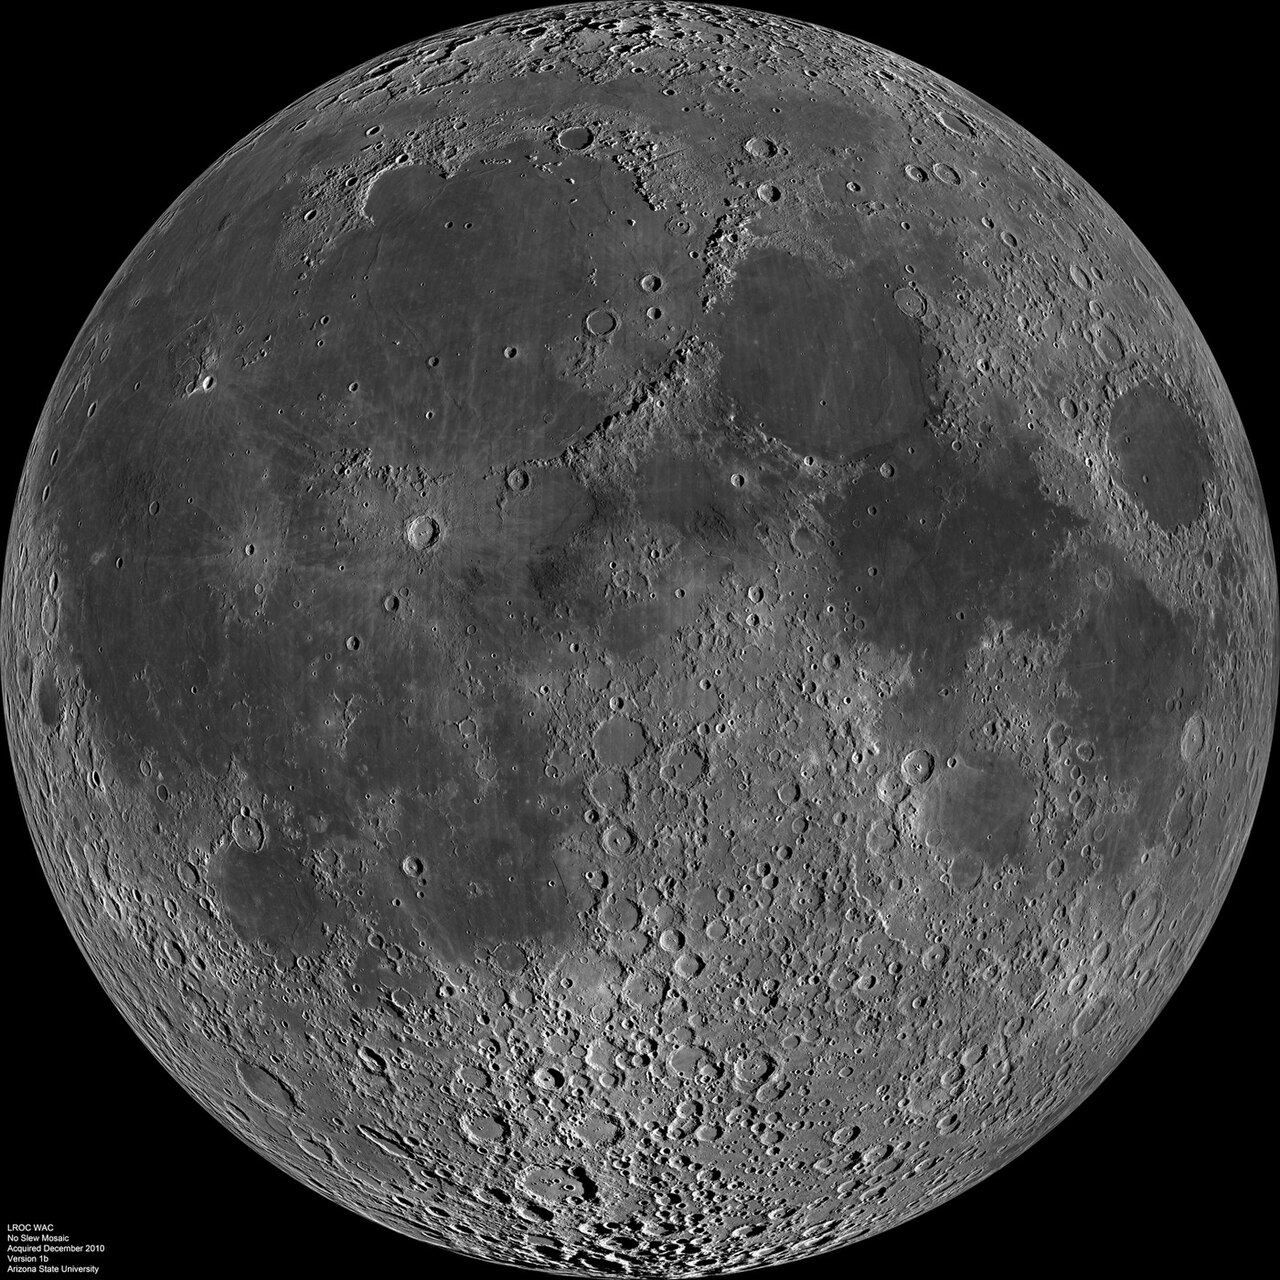
\includegraphics[width=0.44\linewidth]{images/book1/moon-nearside-lro.jpg}

{\small وجه \omterm{def:g2:moon-in-the-sky:moon}{القمر}، مصوَّرًا من المدار: فوّهات على شكل أوعية في كل
مكان، وسهول داكنة واسعة --- ولا \omterm{def:g2:air-around-us:air}{هواء} ولا \omterm{def:g2:air-around-us:wind}{ريح} ولا
صوت. \emph{الصورة: NASA/GSFC/جامعة ولاية أريزونا.}}
\end{omfigure}

\begin{example}[القمر الذي يتبعك]\label{ex:g2:moon-in-the-sky:follows}
امشِ في الشارع في مساء مقمر: تنزلق البيوت والأشجار مبتعدة، لكن
\omterm{def:g2:moon-in-the-sky:moon}{القمر} يبدو تابعًا لك، عند كتفك دائمًا. وهو لا يطاردك حقًّا ---
إنما هو من البعد بحيث لا يغيّر قطعُ شارع كامل منظرَه لك البتة،
بينما تتغيّر البيوت القريبة في كل لحظة. فالأشياء البعيدة جدًّا
تبدو تابعة لكل مسافر؛ \omterm{def:g2:moon-in-the-sky:moon}{والقمر} أحسنها فعلًا لأنه بطل البعد.
\end{example}

\section{ضوء منعكس}

\begin{example}[ضوء القمر ضوء شمس منعكس]\label{ex:g2:moon-in-the-sky:borrowed}
أهو \omterm{def:g1:light-and-shadows:source}{منبع ضوء}؟ تذكّر اختبار السنة الماضية: أيصنع \omterm{def:g1:light-and-shadows:source}{ضوءه} بنفسه؟ لا
--- \omterm{def:g2:moon-in-the-sky:moon}{فالقمر} كرة من صخر داكن، مثل حصاة ضخمة في السماء. وما نسمّيه
\omterm{def:g1:light-and-shadows:source}{ضوء} \omterm{def:g2:moon-in-the-sky:moon}{القمر} ضوءُ شمس \emph{ينعكس} عن ذلك الصخر --- يرتدّ نحونا،
كما يضيء الجدار الأبيض
غرفةً من غير أن يكون مصباحًا. الشمس تضيء \omterm{def:g2:moon-in-the-sky:moon}{القمر} ساطعًا في جهة
واحدة؛ ونحن نرى ما يواجهنا من تلك الجهة المضيئة.
\end{example}

\begin{omfigure}
\begin{tikzpicture}[scale=0.85]
  \fill[omThm] (0.7,1.5) circle (0.45);
  \foreach \a in {0,30,...,330} {
    \draw[omThm] (0.7,1.5) ++(\a:0.62) -- ++(\a:0.26);
  }
  \node[below, font=\small] at (0.7,0.8) {الشمس};
  \draw[thick] (6.8,1.5) circle (1.1);
  \begin{scope}
    \clip (6.8,1.5) circle (1.1);
    \fill[omExo, opacity=0.5] (6.8,0.3) rectangle (8.1,2.7);
  \end{scope}
  \node[below, font=\small] at (6.8,0.1)
    {الجهة المشمسة ساطعة والبعيدة معتمة};
\end{tikzpicture}

{\small الشمس تضيء نصف \omterm{def:g2:moon-in-the-sky:moon}{القمر}، وهو النصف المواجه لها دائمًا. أما
النصف الآخر ففي ليله الخاص.}
\end{omfigure}

\begin{remark}[قمر نهاري]\label{rem:g2:moon-in-the-sky:daytime}
يظنّ كثير من الناس أن \omterm{def:g2:moon-in-the-sky:moon}{القمر} من مخلوقات الليل --- لكن ارفع بصرك في
بعض العصريات فإذا هو هناك، شبح شاحب في السماء الزرقاء! \omterm{def:g2:moon-in-the-sky:moon}{فالقمر}
يسافر حول الأرض وفق جدوله الخاص ولا يعنيه أعندنا نهار أم ليل. وهو
لا يظهر بالنهار إلا أقلّ اعتدادًا بنفسه، حين يملأ وهجُ الشمس
السماء.
\end{remark}

\section{القمر يغيّر شكله}

\begin{example}[أشكال القمر المتغيّرة]\label{ex:g2:moon-in-the-sky:shapes}
راقب \omterm{def:g2:moon-in-the-sky:moon}{القمر} أمسياتٍ كثيرة تجده يغيّر شكله: \emph{هلال}\index{هلال}
رفيع كقُلامة ظفر، ثم نصف دائرة، ثم شكل ممتلئ يكاد يستدير، ثم قرص
\emph{البدر}\index{بدر} الكامل --- ثم يهبط راجعًا، إلى \omterm{ex:g2:moon-in-the-sky:shapes}{هلال} متّجه
في الجهة الأخرى، حتى يبدو \omterm{def:g2:moon-in-the-sky:moon}{القمر} ليلة أو ليلتين وقد اختفى تمامًا.
ويستغرق العرض كله نحو شهر، ثم يعيد نفسه، في وثوق النهار والليل.
\end{example}

\begin{omfigure}
\begin{tikzpicture}[scale=0.85]
  % dark disc for every station, lit part painted over it
  \foreach \x in {0,2.2,4.4,6.6,8.8} {
    \fill[omExo!75] (\x,0) circle (0.8);
  }
  % crescent: lit right edge only
  \begin{scope}
    \clip (2.2,0) circle (0.8);
    \fill[yellow!30] (2.2,-0.85) rectangle (3.05,0.85);
    \fill[omExo!75] (2.2,0) ellipse (0.5 and 0.8);
  \end{scope}
  % half: lit right half
  \begin{scope}
    \clip (4.4,0) circle (0.8);
    \fill[yellow!30] (4.4,-0.85) rectangle (5.25,0.85);
  \end{scope}
  % almost full: dark left sliver only
  \begin{scope}
    \clip (6.6,0) circle (0.8);
    \fill[yellow!30] (6.6,0) circle (0.8);
    \fill[omExo!75] (5.75,-0.85) rectangle (6.6,0.85);
    \fill[yellow!30] (6.6,0) ellipse (0.5 and 0.8);
  \end{scope}
  % full: all lit
  \fill[yellow!30] (8.8,0) circle (0.8);
  \foreach \x in {0,2.2,4.4,6.6,8.8} {
    \draw[thick] (\x,0) circle (0.8);
  }
  \node[below, font=\small] at (0,-1.05) {محاق: مختبئ};
  \node[below, font=\small] at (2.2,-1.05) {هلال};
  \node[below, font=\small] at (4.4,-1.05) {نصف};
  \node[below, font=\small] at (6.6,-1.05) {يكاد يكتمل};
  \node[below, font=\small] at (8.8,-1.05) {بدر};
\end{tikzpicture}

{\small أسبوعان من مراقبة \omterm{def:g2:moon-in-the-sky:moon}{القمر}: ينمو الشكل المضيء ليلة بعد ليلة
من لا شيء إلى القرص الكامل --- ثم يتقلّص راجعًا.}
\end{omfigure}

\begin{omfigure}
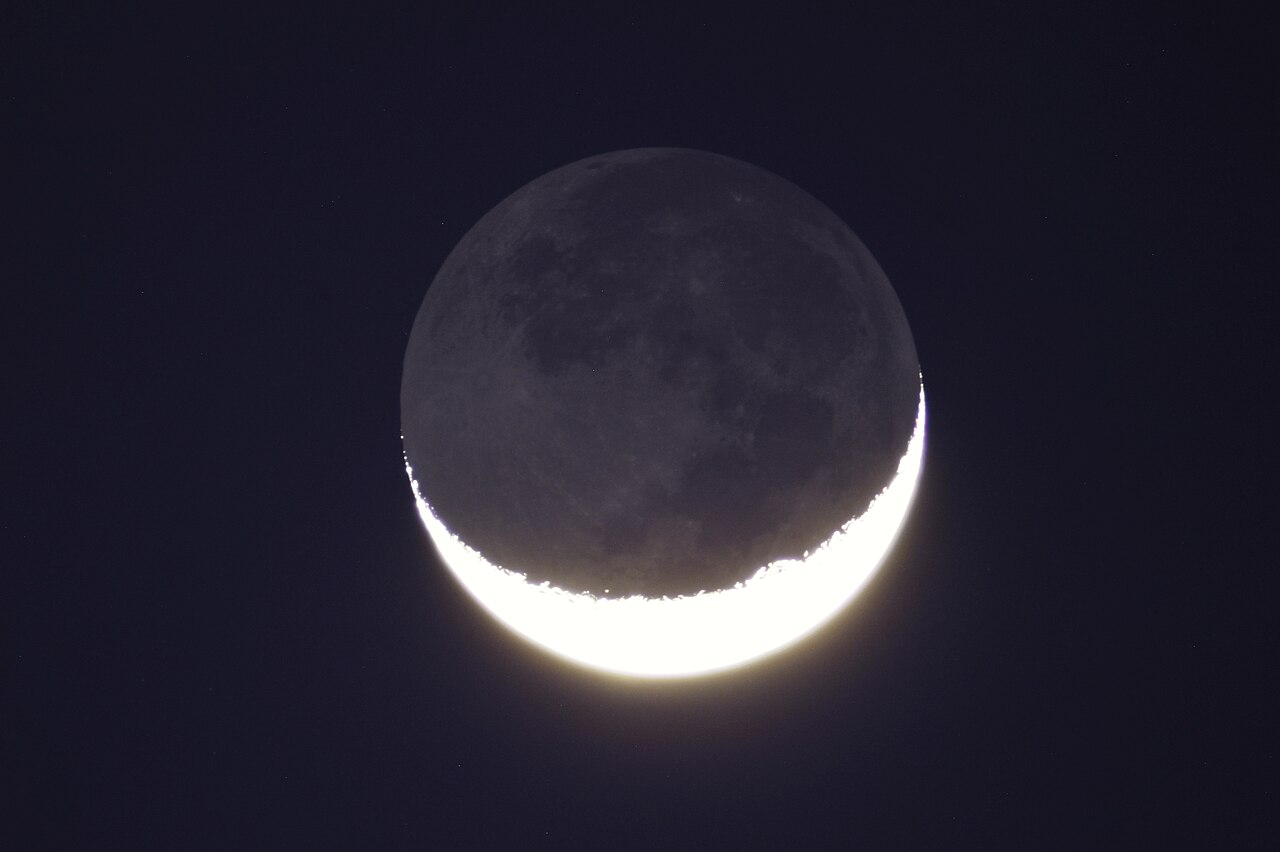
\includegraphics[width=0.42\linewidth]{images/book1/moon-crescent.jpg}\quad
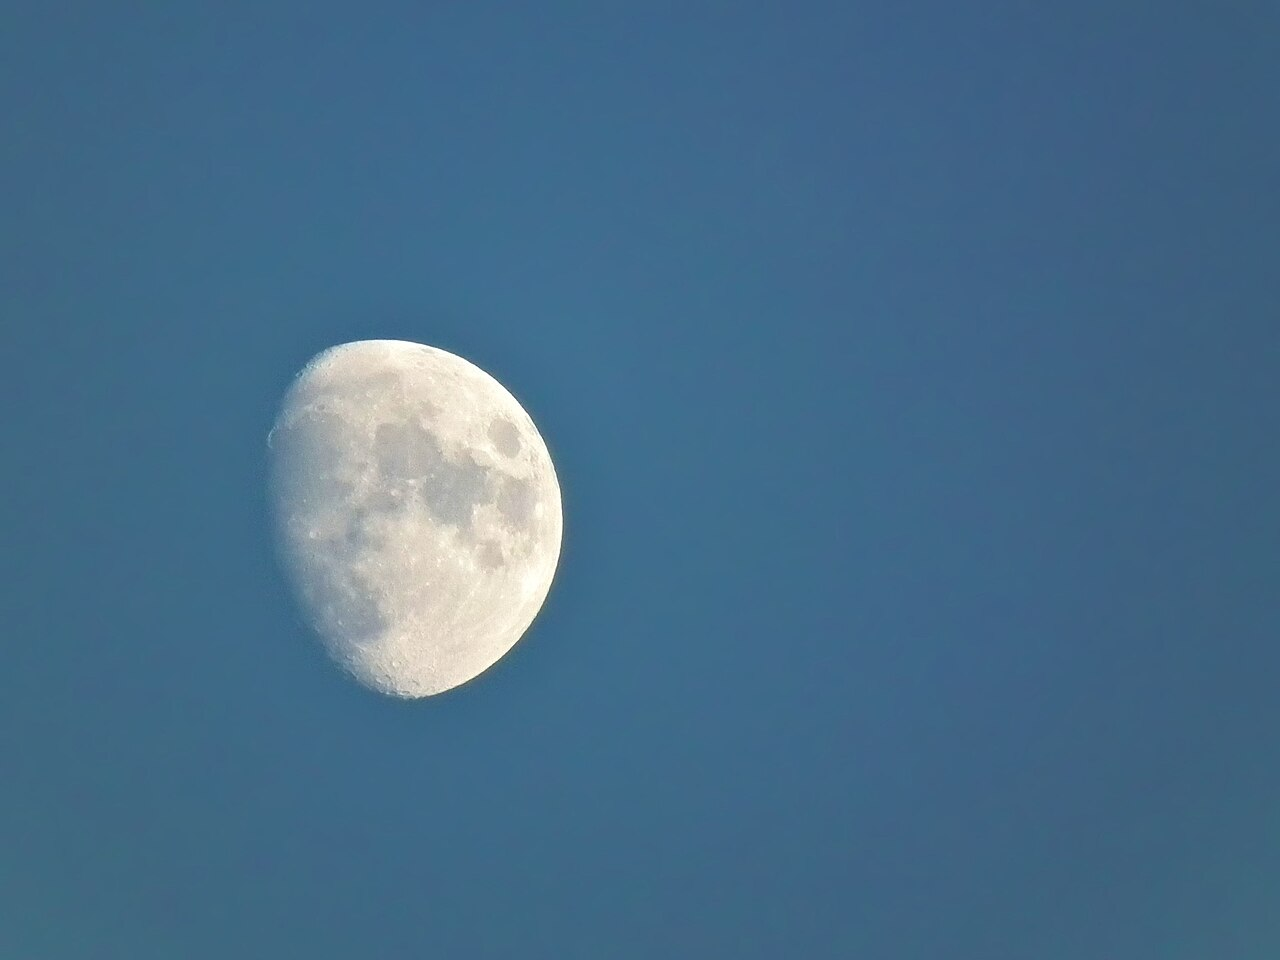
\includegraphics[width=0.42\linewidth]{images/book1/moon-gibbous.jpg}

{\small الحقيقة نفسها: \omterm{ex:g2:moon-in-the-sky:shapes}{هلال} رفيع (على اليسار --- انظر عن قرب:
الجزء المعتم من القرص يتوهّج توهّجًا خافتًا أيضًا) \omterm{def:g2:moon-in-the-sky:moon}{وقمر} يكاد
يكتمل في سماء نهارية (على اليمين). \emph{الصورتان: ج.~دوناتييلو، CC0؛
سيبايل19، CC0.}}
\end{omfigure}

\begin{method}[مفكّرة القمر]\label{met:g2:moon-in-the-sky:diary}
\begin{enumerate}
  \item في كل مساء صافٍ، في الساعة نفسها تقريبًا، ابحث عن
        \omterm{def:g2:moon-in-the-sky:moon}{القمر}؛
  \item ارسم الشكل الذي تراه في مربّع صغير من تقويم --- دائرة،
        وظلّل الجزء المعتم؛
  \item وإن حجبته الغيوم فاكتب ``غيوم'' وواصِل؛
  \item وبعد أسبوعين، صُفّ رسومك في صفّ واحد.
\end{enumerate}
ستبيّن رسومك أنت أن الشكل يتغيّر، قليلًا كل ليلة. أما \emph{لماذا}
يفعل \omterm{def:g2:moon-in-the-sky:moon}{القمر} ذلك فأحجية لذيذة --- وستُحلّ على أصولها في سنة لاحقة
من هذا المنهاج، ومفكّرتك أول خطوة في البرهان.
\end{method}

\section{تمارين}

\begin{exercise}[$\star$]\label{exo:g2:moon-in-the-sky:1}
أالقمر أكبر من الأرض أم أصغر؟ وأقرب من الغيوم أم أبعد؟ وكيف نعلم
أن الناس يستطيعون زيارته؟
\end{exercise}

\begin{exercise}[$\star$]\label{exo:g2:moon-in-the-sky:2}
ما اسم العلامات المستديرة الشبيهة بالأوعية على \omterm{def:g2:moon-in-the-sky:moon}{القمر}، وما الذي
صنعها؟ ولماذا ما زالت هناك بعد كل هذا الزمن؟
\end{exercise}

\begin{exercise}[$\star$]\label{exo:g2:moon-in-the-sky:3}
أالقمر \omterm{def:g1:light-and-shadows:source}{منبع ضوء} مثل المصباح، أم لاقط \omterm{def:g1:light-and-shadows:source}{ضوء} مثل الجدار الأبيض؟ ومن
أين يأتي \omterm{def:g1:light-and-shadows:source}{ضوء} \omterm{def:g2:moon-in-the-sky:moon}{القمر} حقًّا؟
\end{exercise}

\begin{exercise}[$\star$]\label{exo:g2:moon-in-the-sky:4}
أيّ نصف من \omterm{def:g2:moon-in-the-sky:moon}{القمر} تضيئه الشمس: النصف المواجه للشمس دائمًا، أم
النصف نفسه دائمًا، أم نصف مختلف على غير قاعدة؟
\end{exercise}

\begin{exercise}[$\star$]\label{exo:g2:moon-in-the-sky:5}
أيمكن أن يُرى \omterm{def:g2:moon-in-the-sky:moon}{القمر} في النهار؟ وإن قال صديق لا، فما الذي يقنعه؟
\end{exercise}

\begin{exercise}[$\star$]\label{exo:g2:moon-in-the-sky:6}
سمِّ أشكال \omterm{def:g2:moon-in-the-sky:moon}{القمر} بالترتيب، ابتداءً من قُلامة الظفر الرفيعة
وانتهاءً بالفانوس المستدير. وكم يستغرق العرض كله تقريبًا قبل أن
يعيد نفسه؟
\end{exercise}

\begin{exercise}[$\star$]\label{exo:g2:moon-in-the-sky:7}
ليس على \omterm{def:g2:moon-in-the-sky:moon}{القمر} \omterm{def:g2:air-around-us:air}{هواء}. فماذا يحدث لصرخة هناك؟ وللطائرة الورقية؟
\end{exercise}

\begin{exercise}[$\star$]\label{exo:g2:moon-in-the-sky:8}
ابدأ الليلة مفكّرة \omterm{def:g2:moon-in-the-sky:moon}{القمر} في \cref{met:g2:moon-in-the-sky:diary}.
وما الشيئان اللذان يجب أن يبقيا على حالهما كل مساء حتى تكون
المفكّرة عادلة؟
\end{exercise}

\begin{exercise}[$\star\star$]\label{exo:g2:moon-in-the-sky:9}
تقول روزا الصغيرة: ``تبعنا \omterm{def:g2:moon-in-the-sky:moon}{القمر} بسيارتنا إلى البيت كله!'' اشرح
لها، مستعينًا بنزهة الشارع في
\cref{ex:g2:moon-in-the-sky:follows}، لماذا تبدو الأشياء البعيدة
جدًّا تابعة بينما تنزلق القريبة مبتعدة.
\end{exercise}

\begin{exercise}[$\star\star$]\label{exo:g2:moon-in-the-sky:10}
في ليلة \omterm{ex:g2:moon-in-the-sky:shapes}{هلال}، انظر بعناية: يتوهّج الجزء \emph{المعتم} من \omterm{def:g2:moon-in-the-sky:moon}{القمر}
أحيانًا توهّجًا خافتًا جدًّا، حتى تكاد تحزر الدائرة كلها. والشمس
لا تشرق على ذلك الجزء --- لكن شيئًا آخر يشرق قريبًا منه. فأيّ
كرة كبيرة ساطعة تضيئها الشمس يمكن أن تضيء جانب \omterm{def:g2:moon-in-the-sky:moon}{القمر} المعتم، كما
يضيء \omterm{def:g2:moon-in-the-sky:moon}{القمر} لياليَنا؟ (تلميح: أنت واقف عليها.)
\end{exercise}
